%! app: TODOapp
%! outcome: TODOoutcome

\begin{enumerate}
    \item Consider the logic circuit
        \begin{center}
        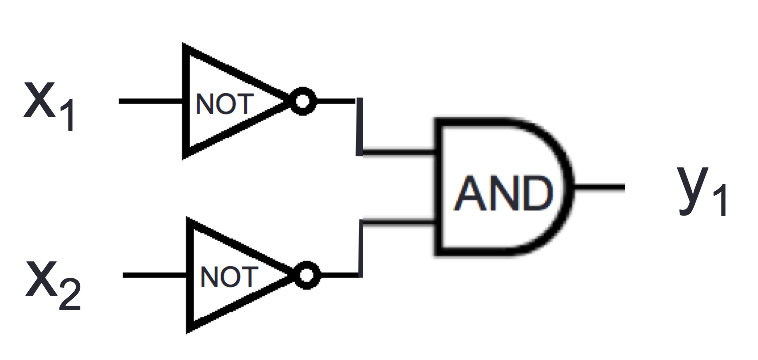
\includegraphics[width=2in]{../../resources/images/review-circuit-1.png}
        \end{center}
        Calculate the value of the output of this circuit ($y_1$) for each of the following settings(s) of input values.
        \begin{enumerate}
            \item $x_1 = 1$, $x_2 = 1$
            \item $x_1 = 1$, $x_2 = 0$
            \item $x_1 = 0$, $x_2 = 1$
            \item $x_1 = 0$, $x_2 = 0$
        \end{enumerate}  \item Consider the logic circuit
        \begin{center}
        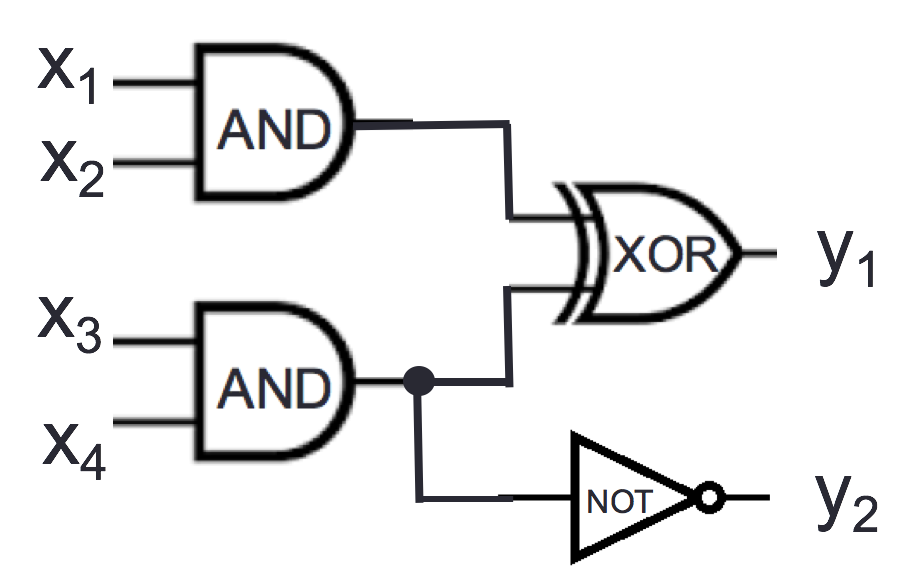
\includegraphics[width=2in]{../../resources/images/review-circuit-2.png}
        \end{center}
        For which of the following settings(s) of input values is the output
        $y_1 = 0$, $y_2 = 1$. (Select all and only those that apply.)
        \begin{enumerate}
            \item $x_1 = 0$, $x_2 = 0$, $x_3 = 0$, and $x_4 = 0$
            \item $x_1 = 1$, $x_2 = 1$, $x_3 = 1$, and $x_4 = 1$
            \item $x_1 = 1$, $x_2 = 0$, $x_3 = 0$, and $x_4 = 1$
            \item $x_1 = 0$, $x_2 = 0$, $x_3 = 1$, and $x_4 = 1$
        \end{enumerate}
      
    \end{enumerate}
    